\documentclass[english]{article}
\usepackage{a4,babel}
\usepackage[utf8]{inputenc}
\usepackage[T1]{fontenc}
\usepackage{graphicx,amssymb,amstext,amsmath,listings,color}
\usepackage{setspace,varioref,url,placeins}

\def\author			{Ludvig Widman(dit06lwn), Emil Eriksson(c07een)}
\def\email			{}
\def\course			{Distributed Systems. 5DV020, HT09}
\def\delivery		{Assignment part 2}
\def\trivialname	{GCom}
\def\tutor			{Lars Larsson, Daniel Henriksson}
\def\myabstract	{}

%-----------------------------------------------------------
\begin{document}
%-----------------------------------------------------------
\begin{titlepage}
\noindent
\course \\
\author \\

\noindent
Tutors: \tutor \\
Date: \today \\
\\
\\
Running the program: 
\begin{verbatim}
$ cd ~dit06lwn/edu/DS/Distsys-Project/
Start registry and sequencer: $ ant seq
Start client: $ ant gui
\end{verbatim}

\begin{center}
	\vspace{20mm}
        \Huge \delivery \\
        \vspace{5mm}
        \Huge \trivialname \\
        \vspace{20mm}
        
\end{center}

\end{titlepage}
%-----------------------------------------------------------
\thispagestyle{empty}
\pagenumbering{roman}
\tableofcontents
\newpage
\pagenumbering{arabic}

\setstretch{1.3}	% Radavstånd
% Mellanrum mellan stycken, inget indrag
\setlength{\parindent}{0pt}
\setlength{\parskip}{1ex plus 0.5ex minus 0.2ex}


%-----------------------------------------------------------
\section{Bonus Level}
We have solved bonus level two with dynamic groups. 


%-----------------------------------------------------------
\section{Tools and language for implementation}
Since the clear recommendation is to use Java and Java RMI we have decided to follow the recommendation. While there are languages that would be more interesting and easier to design GUIs in (cocoa/objective c), Java is more easily ported and the available help from lecturers also helped tip the balance in Java's favor.

JUnit will be used for unit testing and logging will be done through the log4j-package. 

%-----------------------------------------------------------
\section{Project plan}
\begin{tabular}{|l|l|p{7.5cm}|}
\hline
Date	&	Milestone	&	Content \\
\hline
11 Sept	&	Part 1 due	&	Written project plan \\
18 Sept &	Milestone 1 &	Create all interfaces \\ 
						&&	Build dataobjects \\
						&&	Design GUI mockups for test app \\
25 Sept &	Milestone 2 & 	Implement basic methods like non-ordered ordering and non-reliable multicast. \\
2 Oct	&	Milestone 3 & 	Implement advanced methods like total ordering and reliable multicast. \\
9 Oct	&	Milestone 4 & 	Implement GUI-application and debug mode. \\
16 Oct	&	Milestone 5 & 	Resolve distributed problems. \\ && Write on the report.\\ && Make test protocol. \\
23 Oct	&	Finalization 	& Everything should be finished. Minor adjustments. \\
27 Oct	&	Hand in report 	& \\
28-30 Oct & Demonstration	& \\
\hline
\end{tabular}


%-----------------------------------------------------------
\section{Using the demo application}


%-----------------------------------------------------------
\section{System Overview}

\subsection{The gcom package}
The gcom package is the main part of this project. This is where communication, message ordering and group management is handled. 
\subsubsection{GCom}
GCom is the main component in this package and is where the demo application is connected. The application gives commands to GCom, for example create a group or send a message, these commands are translated to messages that GCom sends through the appropriate communication module and to commands to the GroupManagementModule so that the current group state can be maintained.

Information also flows from the communication modules via the message ordering modules back to gcom when messages from other clients is recieved. These messages either effects the group state or is application data that GCom forwards to the application. 

GCom has one GroupManagementModule, one RMIModule and the same amount of communication and message ordering modules as the number of groups it handles.

\subsubsection{BasicCommunicationModule}
The BasicCommunicationModule (BCM) is the simplest implementation of the interface CommunicationModule. It implements basic multicast and has the ability to send and recieve messages. Each communication module corresponds to a specific group. 

When a message is sent the BCM sends it to every member of the group, including the sender. It also detects if the connection is refused to any of the senders and removes these members from the group via a message to GCom.

When the BasicCommunicationModule recieves a message the message is sent directly to the message ordering module for the group.

\subsubsection{ReliableCommunicationModule}
The ReliableCommunicationModule (RCM) extends the BCM and implements reliable multicast.

When the RCM recieves a message it checks if it has recieved it before, if not the message is added to a cache of recieved messages, sent to all group members via BCM and then delivered to message ordering.

Sending messages in the RCM also stores the message in the cache. The message is then sent to all members of the group and the message is delivered to the sender.

When a message is added to the chache, the size of the cache is also trimmed by removing the oldest message if the cache is larger than a specified max size.

\subsubsection{GroupManagementModule}
The GroupManagementModule (GMM) stores information about groups and can notify listeners when something changes.

The main responsabilitys for the GMM includes storing group state, resolving group names to members and updating group state when changes are recieved.

\subsubsection{RMIModule}
The RMIModule connects to a rmi registry at a given host and port. It then supplys an interface for binding, finding, unbinding and rebinding objects.

\subsubsection{momNonOrdered}
The momNonOrdered is the simplest implementation of the MessageOrderingModule (MOM) interface. Every group has a corresponding message ordering module. The type depends on what the creator of the group chose. 

Message ordering is described in detail in section \vref{messageordering}.

\subsubsection{momFIFO}
This message ordering sorts messages in a First In First Out order, in this case this means that messages is delivered in the same order the sender sent them. See section \vref{mo-fifo} for details.


\subsubsection{momCausal}
Causal ordering orders messages according to a happend before relationship. See section \vref{mo-causal} for details.

\subsubsection{momTotal}
Total ordering means that all clients deliver the messages in the exact same order. See section \vref{mo-total} for details.

\subsubsection{ReferenceKeeper}
The ReferenceKeeper is used by GCom only for the group leader. It checks that the rmi registry has the reference to the leaders RemoteObject and trys to rebind it if not. The ReferenceKeeper is run in it's own thread and rechecks the reference in the registry every minute.

\subsubsection{HashVectorClock}


\subsubsection{GroupDefinition}
\subsubsection{RemoteObject}
\subsubsection{Group}
\subsubsection{Member}
\subsubsection{Message}
\subsubsection{Debug}

\subsection{The rmi package}
\subsubsection{Sequencer}
\subsubsection{GroupSequencer}
\subsubsection{SequencerCommunicationModule}
\subsubsection{RMIServer}
\subsubsection{BackdoorOpener}

\subsection{The gui package}
\subsubsection{GroupPanel}
\subsubsection{GUIViewOther}


\begin{figure}
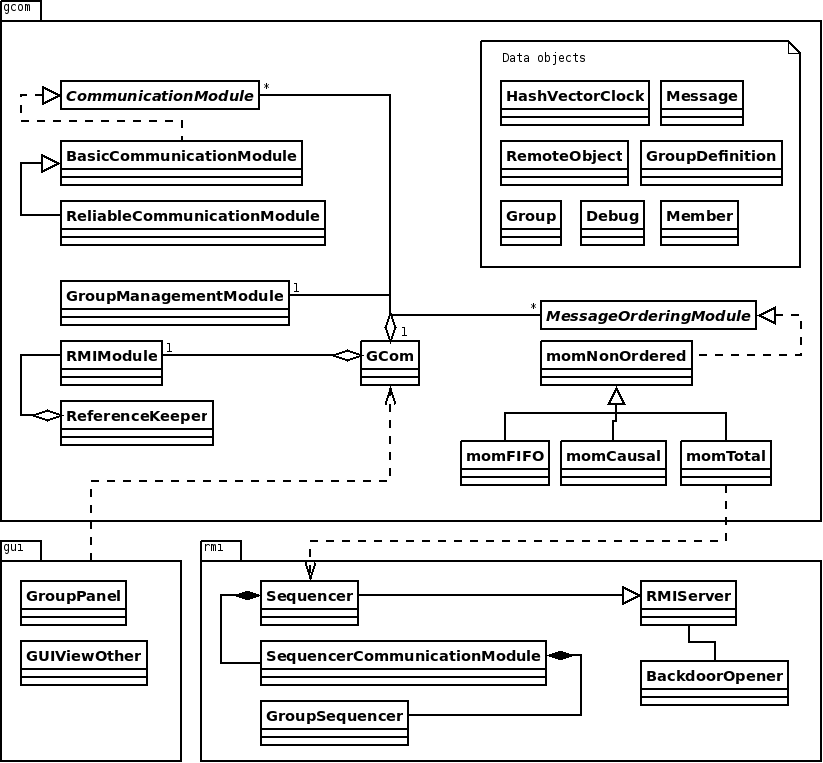
\includegraphics[width=\textwidth]{superuml.png}
\caption{All the classes in the program and an overview of their relations.}
\label{fig:overview}
\end{figure}

%-----------------------------------------------------------
\section{Message ordering and message ordering modules}
\label{messageordering}
GCom features five kinds of message orderings: NonOrdered, FIFO, Causal, Total and CausalTotal. The first four of these has their own message ordering module. Each type of ordering and it's corresponding class is described in detail below.

The message ordering modules have each been thoroghly tested with unit tests to make sure that the algorithms works like intended.

Additional information about algorithms and definitions of the ordering types above can also be found in \cite{distsys-ordering}.

\subsection{Non ordered / momNonOrdered}
The non ordered ordering module (MOM) does not order messages at all. This is the base class for the ordering modules. Every message ordering module has a queing method, a vector clock and message listeners. All the NonOrdered does is to receive messages in the queue method and send them through to it's messages listeners directly. This is also shown in figure \vref{fig:nonorderd}.

The module also has two functions related to the vector clock. It increases the vector clock when told so and returns the clock values if asked. These functions is used in several of the child modules that inherits from momNonOrdered.

\begin{figure}
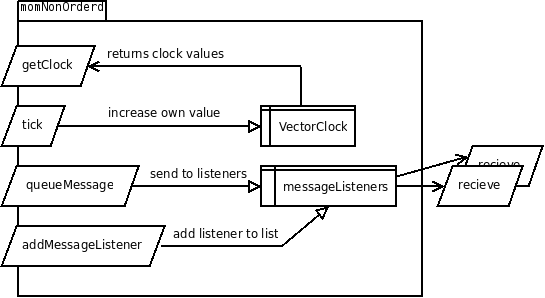
\includegraphics[width=\textwidth]{momNonOrderd.png}
\caption{The non ordered message ordering module just forwards messages to it's listeners. The state of a vector clock is also kept in the module.}
\label{fig:nonorderd}
\end{figure}

\subsection{FIFO ordering / momFIFO}
\label{mo-fifo}
The FIFO ordered MOM delivers messages in the order they where sent. This works by numbering every sent message with a vector clock and storeing recieved messages in a holdback queue until they can be delivered in order. Messages in the queue is compared to the previous last delivered message from the same sender. Messages from new senders is delivered directly as no clockvalue is known. This is also described in figure \vref{fig:fifo}.

In detail the sorting algorithm works as follows:
\begin{enumerate}
\item Check if no previous messages has been recieved from this sender, if so:
	\begin{enumerate}
	\item Send message to message listeners.
	\item Increase local clockvalue for sender by one.
	\end{enumerate}
\item If not, add message to the holdback queue.
\item Loop through the holdback queue and with any message that has a clockvalue that equals the local clockvalue plus one:
	\begin{enumerate}
	\item Send message to message listeners.
	\item Increase local clockvalue for sender by one.
	\item Remove message from holdback queue.
	\end{enumerate}
\end{enumerate}

\begin{figure}
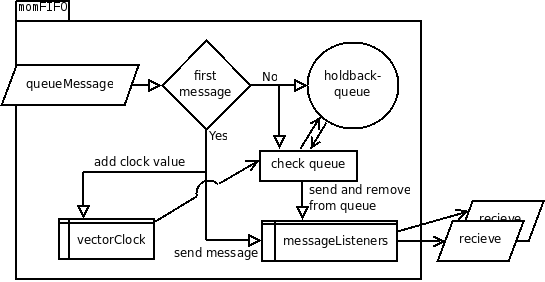
\includegraphics[width=\textwidth]{momFIFO.png}
\caption{The FIFO ordered MOM places messages in a holdback queue until they can be delivered in the order they where sent. Messages from new senders are delivered directly as no previous clockvalue is known.}
\label{fig:fifo}
\end{figure}

\subsection{Causal ordering / momCausal}
\label{mo-causal}
Causal ordering is an ordering where a message can not be delivered before a message that happend before it. Just like in the FIFO ordering the message is first placed in a holdback queue. If a new sender is detected their clockvalue is added to the local clock.

Messages in the queue is checked when a message is recieved. If all previous messages from the same sender has been delivered, and all messages delivered by the sender when the message was timestamped has been delivered, then the message can be delivered. See figure \vref{fig:causal}.

In detail the sorting algorithm works as follows:
\begin{enumerate}
\item Check if no previous messages has been recieved from this sender, if so:\\
	Add senders clockvalue minus one, from message to local clock
\item If not, add message to the holdback queue.
\item Loop through the holdback queue and with any message that:
	\begin{enumerate}
	\item Has a clockvalue for the sender that equals the local clockvalue for the sender plus one
	\item Has clockvalues before or equal to corresponding local clockvalues, excluding the value for the sender
	\end{enumerate}
	Do the following:
	\begin{enumerate}
	\item Send message to message listeners.
	\item Increase local clockvalue for sender by one.
	\item Remove message from holdback queue.
	\end{enumerate}
\end{enumerate}

In step 1 the clockvalue minus one is added to the local clock, this is since the message can not be delivered directly like in FIFO ordering (the message might not conform to criteria b). 

\begin{figure}
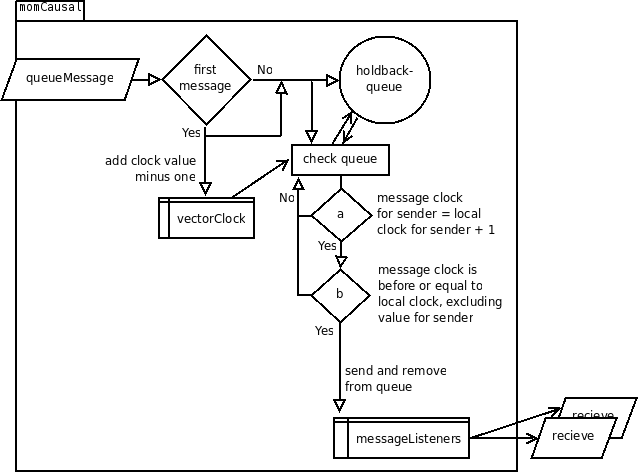
\includegraphics[width=\textwidth]{momCausal.png}
\caption{The Causal ordered MOM places a message in a holdback queue until all messages that happened before it has been deliverd.}
\label{fig:causal}
\end{figure}

\subsection{Total ordering / momTotal}
\label{mo-total}
Total ordering is an ordering where every client delivers the messages in the same order. In our implementation this is solved by the use of a sequencer, which is an appliation that is global for the group. 

When a message is recieved it is sent to the sequencer. The sequencer gives the message a serial number and sends it back. When the MOM get's a message with a serial number it puts it in holdback queue until it can be delivered in sequence (that is until all messages with a lower number is delivered). This is also described in figure \vref{fig:total}.

The first message with a serial number the MOM recieves is delivered directly and any message with a lower number than that is discarded.

\begin{figure}
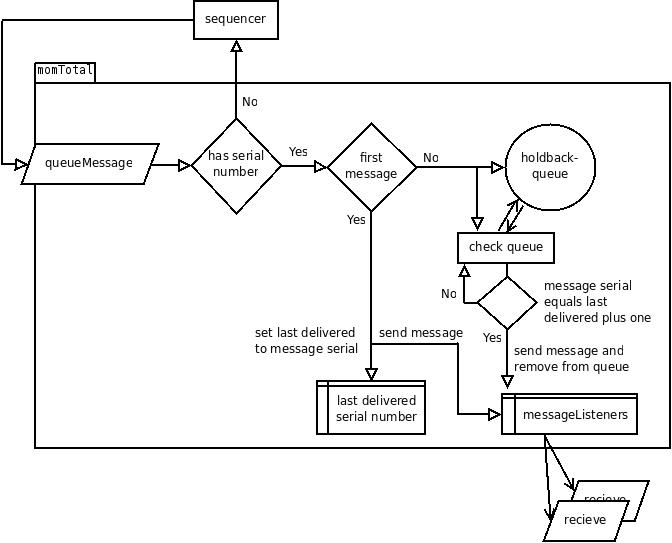
\includegraphics[width=\textwidth]{momTotal.png}
\caption{Total ordering uses a sequencer to deliver messages in the same order in every client.}
\label{fig:total}
\end{figure}

\subsection{Causal total ordering}
Causal total ordering uses the same MOM as total ordering. The only difference is in the sequencer.

With causal total ordering the sequencer uses a momCausal to order the messages in causal order and gives them serial numbers in the order they are delivered. This interaction is shown in figure \vref{fig:totalc}.

\begin{figure}
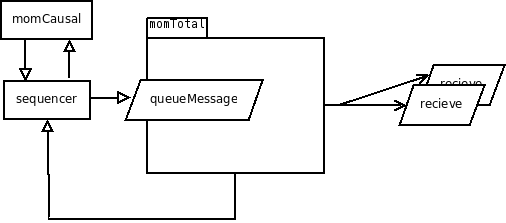
\includegraphics[width=\textwidth]{momTotalC.png}
\caption{Causal total ordering also uses a sequencer, but here the sequencer has a MOM of it's own to give the messages serial numbers in causal order.}
\label{fig:totalc}
\end{figure}

%-----------------------------------------------------------
\section{Design decisions}

\subsection{Selection of bonus level}
We chose to solve bonus level two with dynamic groups since if seemed like an reasonable tradeoff between extra credits and extra workload. 

\subsection{Why an chat Application?}
As our demo application on top of gcom we built a chat application with tabs for different groups. This type of application maps well to the underlying structure of members that belongs to groups. It also gave an easy way to see that messages arrive unharmed and in the correct amount. 

\subsection{Why using a sequencer for total ordering?}
When implementing total ordering one can either use a sequencer or a distributed algorithm. The sequencer method has the downside of the sequencer beeing the single point of failure. However we still choose that method since it seemd mor estraightforward to implement and we already had a single point of failure.

\subsection{Why the sequencer lives in the rmi-server}
The RMI-server has to be setarted before the sequencer and we only wanted a single instance of both so it made sense to put them in the same module (or rather, make the sequencer extend the RMI-server). The RMI-server is also a hopefully quite stable host which makes it a good location for the sequencer.

It would have scaled to more users to put the sequencer in the group leader, but this would make the sequencer less stable (since the group leader might choose to leave the group).

An obvious drawback of having a single sequencer for all groups is that it becomes a bottleneck. This could be solved by moving the sequencer to several dedicated hosts and assigning groups to one of many sequencers.



%-----------------------------------------------------------
\section{Design}
\subsection{GCom}
A framework (middleware) for communicating between distributed nodes within groups.
This module exposes the functionality of the other modules that are part of GCom so that referencing them directly should not be needed in order to use them.
%	(Interface from previous year http://www.cs.umu.se/kurser/5DV020/HT08/GCom.java)

\subsubsection{Interface}
\begin{itemize}
\item[+]  joinGroup(String groupName) \\
	Contact RMI registry and get group-leader \\
	Contact group-leader

\item[+]  createGroup(String groupName)
	Register at RMI registry

\item[+]  removeGroup(String groupName) \\
	Removes the group from the RMI registry

\item[+] leave(String groupName) \\
	Send GroupView excluding sending Member

\item[+]  listGroups \\
	Ask registry

\item[+]  listMembers(String groupName)

\item[+]  sendMessage(String groupName, Message) \\
	Sends a message to the specified group via CommunicationModule

\item[+]  connectToRegistry(String host, int port) \\
	Connects to a RMI registry
\end{itemize}

\subsection{CommunicationModule}
Sends and receives messages to and from other processes. This module must support both reliable and basic multicast. Received data is sent to the MessageOrderingModule. The GroupManagementModule is also notified with the senders process ID. 

\subsubsection{Interface}
\begin{itemize}
\item[+] receive(Message)
	This method is called remotely by other nodes when sending messages to this node.

\item[+] send(Group, Message) \\
	Look up communication type in group \\
	Look up group members

\item[-] multicastB
	Private method used internally to perform a basic multicast.

\item[-] multicastR
	Private method which uses multicastB to perform a reliable multicast.

\end{itemize}

\subsection{MessageOrderingModule}
Sorts incoming messages and makes sure that they're delivered according to the specified order (Non-ordered, FIFO, Causal, Total, Causal-Total). Non-ordered is the main class and the other ordering methods is implemented as subclasses. 

\subsubsection{Interface}
\begin{itemize}
\item[+] queueMessage(Message)
\end{itemize}

\subsection{GroupManagementModule}
The GroupManagementModule contains collection of Group objects. It monitors if a process stops responding. Notifies changes in the states to all members of the group (via the CommunicationModule). The GroupManagementModule also resolves group names to a list of members.

\subsubsection{Interface}
\begin{itemize}
\item[+] addGroup(String groupName)
\item[+] removeGroup(String groupName)
\item[+] listGroups
\end{itemize}

\subsection{Group}
Stores a group's state and group members.

\subsubsection{Interface}
\begin{itemize}
\item[+] addMember \\
	Adds the member to the member list
\item[+]  removeMember \\
	Removes the member from the member list
\item[+]  listMembers
\item[+]  update(ProcessID) \\
	Updates the last seen vector time for the process
\end{itemize}


\subsection{GUI}
The GUI class contains the application that uses GCom and is mostly used for testing and demonstration. We intend to write some kind of simple chat application. The GUI registers listeners in the GCom class to get information. 


\subsection{Message}
The Message is a basic data object which can be serialized. It contains a Vector clock, a destination group, message type and the actual message. 

\subsection{RMI Registry}
A central RMI-registry. Single point of failure. Leader registers and unregisters group. 

\begin{figure}[h]
	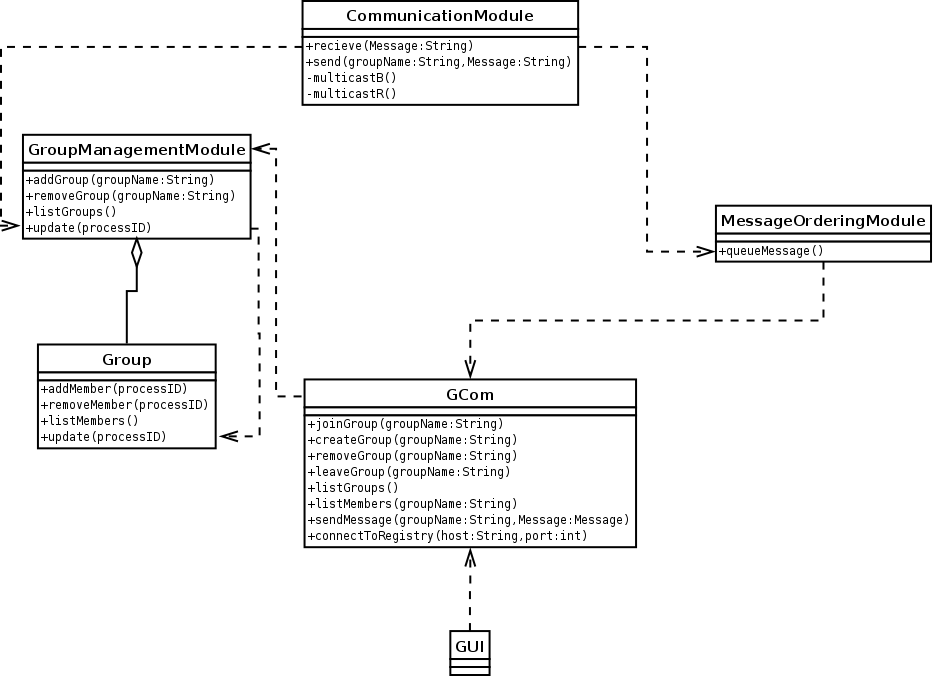
\includegraphics[width=150mm]{klasser.png}
	\caption{How the modules are related.}
\end{figure}

%-----------------------------------------------------------
\section{Use cases}

A few of the scenarios that might arise during using and testing GCom.

\subsection{A node creates a new group}
When a node wants to create a new group, it connects to the RMI-Registry and leaves a reference to itself under the name of the channel.

If this succeeds it sets itself as the group leader and adds itself to it's view of the group in the GroupManagementModule.

If the registration fails an exception indicating if the name was already taken or the RMI-Registry was unresponsive is thrown.

\subsection{A group leader removes a group}
The leader removes all members from it's view of the group in GroupManagementModule and then sends this updated view to all members of the group via the CommunicationModule. It then unregisters the group name in the registry.

\subsection{A member joins a group}
When joining a group the prospective member connects to the RMI-Registry and gets a reference to the group leader and sends it a join request. The leader adds the new member to it's view of the group and then sends this updated view to all members of the group, including the new member. When the new member receives the updated view it knows it is part of the group.

\subsection{A member leaves group}
When a member wants to leave a group it sends a group view excluding itself to all the members (including the group-leader) of the group.

\subsection{Send message to a group}
First a list of all members in the group is obtained from the GroupManagementModule and then the message is sent to all of the members.

%\subsection{Member receives message with much later time-stamp than previous message}
%TODO: Design a way for a node to request an older message

\subsection{Group-leader leaves group}
When the group-leader leaves the group the remaining members starts electing a new group leader by creating a semi-random (and unique) value and sending this to all other nodes in an election-message.

%TODO: A crashed node could make a group-leader election fail.
When a node receives election-messages it compares the value in the incoming message with the value it created and sends the larger of these to all other nodes. When a node has received messages with it's own value from all members of the group it sets itself as group-leader and registers with the RMI-Registry.

For now we do not take into account that a node might crash during the election.

If the group-leader leaves a single member behind this node realizes it is alone in the group and sets itself as group-leader and registers with the registry.

\subsection{The last member in a group leaves}
When the last member of a group leaves it is the group-leader and it unregisters itself from the registry.

%-----------------------------------------------------------
\section{Fault tolerance}

\subsection{Detecting crashed members}
The GroupManagementModule gets notified when a message is received and can therefore keep track of the time since the last message from a process, measured in vector time. If a process does not send anything for a long time it will be marked as crashed and removed from the group list.

\subsection{If the registry restarts or is unresponsive}
The leader of each group occasionally checks that the group is registered in the RMI-registry. If the registry has restarted for some reason the leader will re-register the group.

\subsection{If the group leader crashes}
If the group leader crashes the group will detect that no messages arrive from the leader and then elect a new leader. 

\subsection{If the last member of a group crashes}
If the last member of a group crashes no one will unregister the group.
This will potentially lead to a lot of "dead" references in the registry if there is a bug causing nodes to crash when they are the last to leave a group. In order to counter this some extra testing will be done to make sure that nodes behave when leaving and unregistering with the registry.
If the time allows we will try to implement a way to clear out old references in the registry (other than restarting it periodically).

\subsection{Netsplit}
If the group is split in two partitions, due to a cable failure or similar, the partition with the leader will continue to work as before. The other partition will elect a new leader when they discover that they no longer receive messages from the leader.
The new leader will try to reregister the group in the registry. The leader for the other part will do the same and therefore compete over the reference in the registry. Because of this newcomers will join the group having the reference in the registry at the time the node connects.

%-----------------------------------------------------------
\section{Requirement Specification}

\subsection{Group management}
\begin{description}
\item[REQUIRED] External processes must be able to find and connect to group leaders via a RMI registry.

\item[REQUIRED] The group leader must regularly make sure that the group and leader is registered in the RMI registry.

\item[REQUIRED] Any process must be able to create a new group and register itself as leader in the registry.

\item[REQUIRED] Any process must be able to join a group by connecting to the group leader.

\item[REQUIRED] Every process in a group must notify the other processes of any known changes to the group composition.

\item[REQUIRED] Every process must keep track of the members of all the groups it's a member of.

\item[REQUIRED] Every process must monitor if another process in the group stops responding and report a corresponding change in group composition.

\item[REQUIRED] If the leader of the group leaves or crashes a new leader must be elected in the group.
\end{description}


\subsection{Communication}
\begin{description}
\item[REQUIRED] It must be possible to send messages to the members of joined group.

\item[REQUIRED] Both non-reliable and reliable multicast must be supported for sending messages.

\item[REQUIRED] The communication method chosen by the group creator (reliable or non-reliable multicast) must be used when communicating in a group.

\item[REQUIRED] Every message must contain a updated vector clock.
\end{description}


\subsection{Message Ordering}
\begin{description}
\item[REQUIRED] Any message must arrive in proper order (according to the selected sorting requirements).

\item[REQUIRED] A message must not be delivered until all previous messages are delivered if the message ordering demands so.
\end{description}



%-----------------------------------------------------------
\section{Limitations}
\begin{itemize}
\item The RMI-registry is a single point of failure. If the registry crashes no processes can find or join groups. 

\item If a group is split in two parts due to network failure and both parts still have contact  with the registry bad things will happen. This is assumed to never happen.

\item All processes are assumed to be good. If a process starts to lie or send malicious messages bad things will happen.
\end{itemize}

\begin{thebibliography}{5}

\bibitem{distsys-ordering} Distributed systems : concepts and design / GeorgeCoulouris, Jean Dollimore, Tim Kondberg.--4th ed. p. 490-498

\end{thebibliography}



\end{document}
